% Created by tikzDevice version 0.12.3.1 on 2023-04-07 21:24:40
% !TEX encoding = UTF-8 Unicode
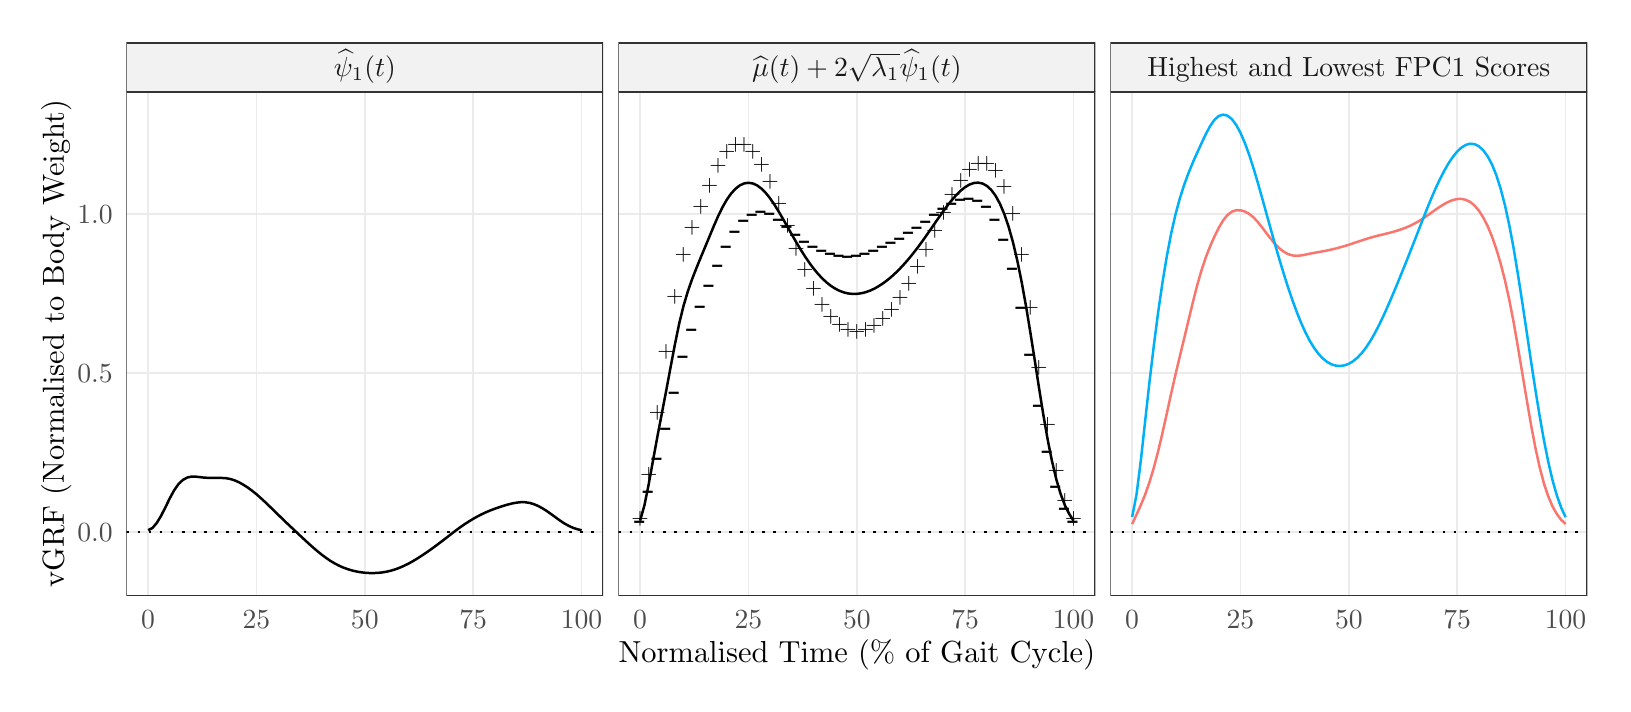
\begin{tikzpicture}[x=1pt,y=1pt]
\definecolor{fillColor}{RGB}{255,255,255}
\path[use as bounding box,fill=fillColor,fill opacity=0.00] (0,0) rectangle (569.05,237.11);
\begin{scope}
\path[clip] (  0.00,  0.00) rectangle (569.05,237.11);
\definecolor{drawColor}{RGB}{255,255,255}
\definecolor{fillColor}{RGB}{255,255,255}

\path[draw=drawColor,line width= 0.6pt,line join=round,line cap=round,fill=fillColor] (  0.00,  0.00) rectangle (569.05,237.11);
\end{scope}
\begin{scope}
\path[clip] ( 35.69, 31.75) rectangle (207.98,213.97);
\definecolor{fillColor}{RGB}{255,255,255}

\path[fill=fillColor] ( 35.69, 31.75) rectangle (207.98,213.97);
\definecolor{drawColor}{gray}{0.92}

\path[draw=drawColor,line width= 0.6pt,line join=round] ( 35.69, 54.87) --
	(207.98, 54.87);

\path[draw=drawColor,line width= 0.6pt,line join=round] ( 35.69,112.36) --
	(207.98,112.36);

\path[draw=drawColor,line width= 0.6pt,line join=round] ( 35.69,169.85) --
	(207.98,169.85);

\path[draw=drawColor,line width= 0.6pt,line join=round] ( 43.52, 31.75) --
	( 43.52,213.97);

\path[draw=drawColor,line width= 0.6pt,line join=round] ( 82.68, 31.75) --
	( 82.68,213.97);

\path[draw=drawColor,line width= 0.6pt,line join=round] (121.83, 31.75) --
	(121.83,213.97);

\path[draw=drawColor,line width= 0.6pt,line join=round] (160.99, 31.75) --
	(160.99,213.97);

\path[draw=drawColor,line width= 0.6pt,line join=round] (200.15, 31.75) --
	(200.15,213.97);
\definecolor{drawColor}{RGB}{0,0,0}

\path[draw=drawColor,line width= 0.9pt,line join=round] ( 43.52, 55.53) --
	( 45.09, 56.31) --
	( 46.65, 58.14) --
	( 48.22, 60.75) --
	( 49.79, 63.84) --
	( 51.35, 67.04) --
	( 52.92, 69.93) --
	( 54.48, 72.16) --
	( 56.05, 73.66) --
	( 57.62, 74.53) --
	( 59.18, 74.89) --
	( 60.75, 74.87) --
	( 62.32, 74.69) --
	( 63.88, 74.51) --
	( 65.45, 74.43) --
	( 67.01, 74.40) --
	( 68.58, 74.41) --
	( 70.15, 74.40) --
	( 71.71, 74.30) --
	( 73.28, 74.01) --
	( 74.85, 73.51) --
	( 76.41, 72.81) --
	( 77.98, 71.93) --
	( 79.54, 70.92) --
	( 81.11, 69.77) --
	( 82.68, 68.51) --
	( 84.24, 67.13) --
	( 85.81, 65.68) --
	( 87.38, 64.17) --
	( 88.94, 62.65) --
	( 90.51, 61.12) --
	( 92.07, 59.60) --
	( 93.64, 58.09) --
	( 95.21, 56.61) --
	( 96.77, 55.14) --
	( 98.34, 53.66) --
	( 99.91, 52.20) --
	(101.47, 50.76) --
	(103.04, 49.36) --
	(104.60, 48.01) --
	(106.17, 46.74) --
	(107.74, 45.57) --
	(109.30, 44.50) --
	(110.87, 43.56) --
	(112.44, 42.74) --
	(114.00, 42.04) --
	(115.57, 41.47) --
	(117.13, 40.99) --
	(118.70, 40.62) --
	(120.27, 40.34) --
	(121.83, 40.15) --
	(123.40, 40.05) --
	(124.97, 40.03) --
	(126.53, 40.10) --
	(128.10, 40.26) --
	(129.66, 40.52) --
	(131.23, 40.89) --
	(132.80, 41.36) --
	(134.36, 41.94) --
	(135.93, 42.62) --
	(137.50, 43.39) --
	(139.06, 44.25) --
	(140.63, 45.19) --
	(142.19, 46.18) --
	(143.76, 47.23) --
	(145.33, 48.32) --
	(146.89, 49.45) --
	(148.46, 50.62) --
	(150.03, 51.80) --
	(151.59, 53.01) --
	(153.16, 54.22) --
	(154.72, 55.42) --
	(156.29, 56.57) --
	(157.86, 57.66) --
	(159.42, 58.68) --
	(160.99, 59.63) --
	(162.56, 60.51) --
	(164.12, 61.31) --
	(165.69, 62.04) --
	(167.25, 62.69) --
	(168.82, 63.28) --
	(170.39, 63.83) --
	(171.95, 64.34) --
	(173.52, 64.80) --
	(175.09, 65.19) --
	(176.65, 65.48) --
	(178.22, 65.64) --
	(179.78, 65.62) --
	(181.35, 65.39) --
	(182.92, 64.93) --
	(184.48, 64.26) --
	(186.05, 63.41) --
	(187.62, 62.42) --
	(189.18, 61.32) --
	(190.75, 60.17) --
	(192.31, 59.05) --
	(193.88, 58.00) --
	(195.45, 57.11) --
	(197.01, 56.41) --
	(198.58, 55.89) --
	(200.15, 55.49);

\path[draw=drawColor,line width= 0.6pt,dash pattern=on 1pt off 3pt ,line join=round] ( 35.69, 54.87) -- (207.98, 54.87);
\definecolor{drawColor}{gray}{0.20}

\path[draw=drawColor,line width= 0.6pt,line join=round,line cap=round] ( 35.69, 31.75) rectangle (207.98,213.97);
\end{scope}
\begin{scope}
\path[clip] (213.48, 31.75) rectangle (385.77,213.97);
\definecolor{fillColor}{RGB}{255,255,255}

\path[fill=fillColor] (213.48, 31.75) rectangle (385.77,213.97);
\definecolor{drawColor}{gray}{0.92}

\path[draw=drawColor,line width= 0.6pt,line join=round] (213.48, 54.87) --
	(385.77, 54.87);

\path[draw=drawColor,line width= 0.6pt,line join=round] (213.48,112.36) --
	(385.77,112.36);

\path[draw=drawColor,line width= 0.6pt,line join=round] (213.48,169.85) --
	(385.77,169.85);

\path[draw=drawColor,line width= 0.6pt,line join=round] (221.31, 31.75) --
	(221.31,213.97);

\path[draw=drawColor,line width= 0.6pt,line join=round] (260.47, 31.75) --
	(260.47,213.97);

\path[draw=drawColor,line width= 0.6pt,line join=round] (299.62, 31.75) --
	(299.62,213.97);

\path[draw=drawColor,line width= 0.6pt,line join=round] (338.78, 31.75) --
	(338.78,213.97);

\path[draw=drawColor,line width= 0.6pt,line join=round] (377.93, 31.75) --
	(377.93,213.97);
\definecolor{drawColor}{RGB}{0,0,0}

\path[draw=drawColor,line width= 0.9pt,line join=round] (221.31, 58.99) --
	(222.87, 64.55) --
	(224.44, 72.30) --
	(226.01, 80.97) --
	(227.57, 89.46) --
	(229.14, 97.65) --
	(230.71,105.83) --
	(232.27,114.20) --
	(233.84,122.46) --
	(235.40,130.07) --
	(236.97,136.52) --
	(238.54,141.80) --
	(240.10,146.27) --
	(241.67,150.30) --
	(243.24,154.14) --
	(244.80,157.88) --
	(246.37,161.65) --
	(247.93,165.41) --
	(249.50,169.01) --
	(251.07,172.23) --
	(252.63,174.96) --
	(254.20,177.19) --
	(255.77,178.90) --
	(257.33,180.12) --
	(258.90,180.83) --
	(260.47,181.06) --
	(262.03,180.81) --
	(263.60,180.11) --
	(265.16,178.95) --
	(266.73,177.36) --
	(268.30,175.39) --
	(269.86,173.11) --
	(271.43,170.58) --
	(273.00,167.89) --
	(274.56,165.12) --
	(276.13,162.34) --
	(277.69,159.63) --
	(279.26,157.01) --
	(280.83,154.53) --
	(282.39,152.23) --
	(283.96,150.12) --
	(285.53,148.21) --
	(287.09,146.53) --
	(288.66,145.07) --
	(290.22,143.83) --
	(291.79,142.82) --
	(293.36,142.03) --
	(294.92,141.45) --
	(296.49,141.07) --
	(298.06,140.90) --
	(299.62,140.92) --
	(301.19,141.13) --
	(302.75,141.51) --
	(304.32,142.07) --
	(305.89,142.78) --
	(307.45,143.66) --
	(309.02,144.68) --
	(310.59,145.84) --
	(312.15,147.14) --
	(313.72,148.58) --
	(315.28,150.14) --
	(316.85,151.83) --
	(318.42,153.63) --
	(319.98,155.56) --
	(321.55,157.59) --
	(323.12,159.71) --
	(324.68,161.91) --
	(326.25,164.17) --
	(327.81,166.45) --
	(329.38,168.71) --
	(330.95,170.91) --
	(332.51,173.02) --
	(334.08,174.98) --
	(335.65,176.74) --
	(337.21,178.27) --
	(338.78,179.51) --
	(340.34,180.43) --
	(341.91,180.98) --
	(343.48,181.12) --
	(345.04,180.79) --
	(346.61,179.93) --
	(348.18,178.49) --
	(349.74,176.37) --
	(351.31,173.52) --
	(352.87,169.84) --
	(354.44,165.24) --
	(356.01,159.66) --
	(357.57,153.06) --
	(359.14,145.37) --
	(360.71,136.70) --
	(362.27,127.28) --
	(363.84,117.35) --
	(365.40,107.24) --
	(366.97, 97.44) --
	(368.54, 88.45) --
	(370.10, 80.62) --
	(371.67, 74.00) --
	(373.24, 68.65) --
	(374.80, 64.51) --
	(376.37, 61.37) --
	(377.93, 58.97);

\node[text=drawColor,anchor=base,inner sep=0pt, outer sep=0pt, scale=  0.81] at (221.31, 57.60) {+};

\node[text=drawColor,anchor=base,inner sep=0pt, outer sep=0pt, scale=  0.81] at (224.44, 73.34) {+};

\node[text=drawColor,anchor=base,inner sep=0pt, outer sep=0pt, scale=  0.81] at (227.57, 95.78) {+};

\node[text=drawColor,anchor=base,inner sep=0pt, outer sep=0pt, scale=  0.81] at (230.71,117.82) {+};

\node[text=drawColor,anchor=base,inner sep=0pt, outer sep=0pt, scale=  0.81] at (233.84,137.91) {+};

\node[text=drawColor,anchor=base,inner sep=0pt, outer sep=0pt, scale=  0.81] at (236.97,153.11) {+};

\node[text=drawColor,anchor=base,inner sep=0pt, outer sep=0pt, scale=  0.81] at (240.10,162.67) {+};

\node[text=drawColor,anchor=base,inner sep=0pt, outer sep=0pt, scale=  0.81] at (243.24,170.30) {+};

\node[text=drawColor,anchor=base,inner sep=0pt, outer sep=0pt, scale=  0.81] at (246.37,177.80) {+};

\node[text=drawColor,anchor=base,inner sep=0pt, outer sep=0pt, scale=  0.81] at (249.50,185.05) {+};

\node[text=drawColor,anchor=base,inner sep=0pt, outer sep=0pt, scale=  0.81] at (252.63,190.27) {+};

\node[text=drawColor,anchor=base,inner sep=0pt, outer sep=0pt, scale=  0.81] at (255.77,192.75) {+};

\node[text=drawColor,anchor=base,inner sep=0pt, outer sep=0pt, scale=  0.81] at (258.90,192.67) {+};

\node[text=drawColor,anchor=base,inner sep=0pt, outer sep=0pt, scale=  0.81] at (262.03,190.20) {+};

\node[text=drawColor,anchor=base,inner sep=0pt, outer sep=0pt, scale=  0.81] at (265.16,185.58) {+};

\node[text=drawColor,anchor=base,inner sep=0pt, outer sep=0pt, scale=  0.81] at (268.30,179.18) {+};

\node[text=drawColor,anchor=base,inner sep=0pt, outer sep=0pt, scale=  0.81] at (271.43,171.57) {+};

\node[text=drawColor,anchor=base,inner sep=0pt, outer sep=0pt, scale=  0.81] at (274.56,163.35) {+};

\node[text=drawColor,anchor=base,inner sep=0pt, outer sep=0pt, scale=  0.81] at (277.69,155.13) {+};

\node[text=drawColor,anchor=base,inner sep=0pt, outer sep=0pt, scale=  0.81] at (280.83,147.40) {+};

\node[text=drawColor,anchor=base,inner sep=0pt, outer sep=0pt, scale=  0.81] at (283.96,140.55) {+};

\node[text=drawColor,anchor=base,inner sep=0pt, outer sep=0pt, scale=  0.81] at (287.09,134.89) {+};

\node[text=drawColor,anchor=base,inner sep=0pt, outer sep=0pt, scale=  0.81] at (290.22,130.55) {+};

\node[text=drawColor,anchor=base,inner sep=0pt, outer sep=0pt, scale=  0.81] at (293.36,127.56) {+};

\node[text=drawColor,anchor=base,inner sep=0pt, outer sep=0pt, scale=  0.81] at (296.49,125.82) {+};

\node[text=drawColor,anchor=base,inner sep=0pt, outer sep=0pt, scale=  0.81] at (299.62,125.24) {+};

\node[text=drawColor,anchor=base,inner sep=0pt, outer sep=0pt, scale=  0.81] at (302.75,125.71) {+};

\node[text=drawColor,anchor=base,inner sep=0pt, outer sep=0pt, scale=  0.81] at (305.89,127.20) {+};

\node[text=drawColor,anchor=base,inner sep=0pt, outer sep=0pt, scale=  0.81] at (309.02,129.68) {+};

\node[text=drawColor,anchor=base,inner sep=0pt, outer sep=0pt, scale=  0.81] at (312.15,133.12) {+};

\node[text=drawColor,anchor=base,inner sep=0pt, outer sep=0pt, scale=  0.81] at (315.28,137.47) {+};

\node[text=drawColor,anchor=base,inner sep=0pt, outer sep=0pt, scale=  0.81] at (318.42,142.63) {+};

\node[text=drawColor,anchor=base,inner sep=0pt, outer sep=0pt, scale=  0.81] at (321.55,148.48) {+};

\node[text=drawColor,anchor=base,inner sep=0pt, outer sep=0pt, scale=  0.81] at (324.68,154.87) {+};

\node[text=drawColor,anchor=base,inner sep=0pt, outer sep=0pt, scale=  0.81] at (327.81,161.59) {+};

\node[text=drawColor,anchor=base,inner sep=0pt, outer sep=0pt, scale=  0.81] at (330.95,168.30) {+};

\node[text=drawColor,anchor=base,inner sep=0pt, outer sep=0pt, scale=  0.81] at (334.08,174.54) {+};

\node[text=drawColor,anchor=base,inner sep=0pt, outer sep=0pt, scale=  0.81] at (337.21,179.80) {+};

\node[text=drawColor,anchor=base,inner sep=0pt, outer sep=0pt, scale=  0.81] at (340.34,183.66) {+};

\node[text=drawColor,anchor=base,inner sep=0pt, outer sep=0pt, scale=  0.81] at (343.48,185.77) {+};

\node[text=drawColor,anchor=base,inner sep=0pt, outer sep=0pt, scale=  0.81] at (346.61,185.74) {+};

\node[text=drawColor,anchor=base,inner sep=0pt, outer sep=0pt, scale=  0.81] at (349.74,183.16) {+};

\node[text=drawColor,anchor=base,inner sep=0pt, outer sep=0pt, scale=  0.81] at (352.87,177.41) {+};

\node[text=drawColor,anchor=base,inner sep=0pt, outer sep=0pt, scale=  0.81] at (356.01,167.66) {+};

\node[text=drawColor,anchor=base,inner sep=0pt, outer sep=0pt, scale=  0.81] at (359.14,153.14) {+};

\node[text=drawColor,anchor=base,inner sep=0pt, outer sep=0pt, scale=  0.81] at (362.27,134.00) {+};

\node[text=drawColor,anchor=base,inner sep=0pt, outer sep=0pt, scale=  0.81] at (365.40,112.24) {+};

\node[text=drawColor,anchor=base,inner sep=0pt, outer sep=0pt, scale=  0.81] at (368.54, 91.37) {+};

\node[text=drawColor,anchor=base,inner sep=0pt, outer sep=0pt, scale=  0.81] at (371.67, 74.90) {+};

\node[text=drawColor,anchor=base,inner sep=0pt, outer sep=0pt, scale=  0.81] at (374.80, 63.94) {+};

\node[text=drawColor,anchor=base,inner sep=0pt, outer sep=0pt, scale=  0.81] at (377.93, 57.53) {+};

\node[text=drawColor,anchor=base,inner sep=0pt, outer sep=0pt, scale=  1.37] at (221.31, 55.41) {-};

\node[text=drawColor,anchor=base,inner sep=0pt, outer sep=0pt, scale=  1.37] at (224.44, 66.30) {-};

\node[text=drawColor,anchor=base,inner sep=0pt, outer sep=0pt, scale=  1.37] at (227.57, 78.16) {-};

\node[text=drawColor,anchor=base,inner sep=0pt, outer sep=0pt, scale=  1.37] at (230.71, 88.88) {-};

\node[text=drawColor,anchor=base,inner sep=0pt, outer sep=0pt, scale=  1.37] at (233.84,102.04) {-};

\node[text=drawColor,anchor=base,inner sep=0pt, outer sep=0pt, scale=  1.37] at (236.97,114.96) {-};

\node[text=drawColor,anchor=base,inner sep=0pt, outer sep=0pt, scale=  1.37] at (240.10,124.89) {-};

\node[text=drawColor,anchor=base,inner sep=0pt, outer sep=0pt, scale=  1.37] at (243.24,133.00) {-};

\node[text=drawColor,anchor=base,inner sep=0pt, outer sep=0pt, scale=  1.37] at (246.37,140.52) {-};

\node[text=drawColor,anchor=base,inner sep=0pt, outer sep=0pt, scale=  1.37] at (249.50,147.99) {-};

\node[text=drawColor,anchor=base,inner sep=0pt, outer sep=0pt, scale=  1.37] at (252.63,154.68) {-};

\node[text=drawColor,anchor=base,inner sep=0pt, outer sep=0pt, scale=  1.37] at (255.77,160.08) {-};

\node[text=drawColor,anchor=base,inner sep=0pt, outer sep=0pt, scale=  1.37] at (258.90,164.02) {-};

\node[text=drawColor,anchor=base,inner sep=0pt, outer sep=0pt, scale=  1.37] at (262.03,166.46) {-};

\node[text=drawColor,anchor=base,inner sep=0pt, outer sep=0pt, scale=  1.37] at (265.16,167.34) {-};

\node[text=drawColor,anchor=base,inner sep=0pt, outer sep=0pt, scale=  1.37] at (268.30,166.62) {-};

\node[text=drawColor,anchor=base,inner sep=0pt, outer sep=0pt, scale=  1.37] at (271.43,164.62) {-};

\node[text=drawColor,anchor=base,inner sep=0pt, outer sep=0pt, scale=  1.37] at (274.56,161.91) {-};

\node[text=drawColor,anchor=base,inner sep=0pt, outer sep=0pt, scale=  1.37] at (277.69,159.14) {-};

\node[text=drawColor,anchor=base,inner sep=0pt, outer sep=0pt, scale=  1.37] at (280.83,156.69) {-};

\node[text=drawColor,anchor=base,inner sep=0pt, outer sep=0pt, scale=  1.37] at (283.96,154.71) {-};

\node[text=drawColor,anchor=base,inner sep=0pt, outer sep=0pt, scale=  1.37] at (287.09,153.20) {-};

\node[text=drawColor,anchor=base,inner sep=0pt, outer sep=0pt, scale=  1.37] at (290.22,152.14) {-};

\node[text=drawColor,anchor=base,inner sep=0pt, outer sep=0pt, scale=  1.37] at (293.36,151.52) {-};

\node[text=drawColor,anchor=base,inner sep=0pt, outer sep=0pt, scale=  1.37] at (296.49,151.35) {-};

\node[text=drawColor,anchor=base,inner sep=0pt, outer sep=0pt, scale=  1.37] at (299.62,151.63) {-};

\node[text=drawColor,anchor=base,inner sep=0pt, outer sep=0pt, scale=  1.37] at (302.75,152.34) {-};

\node[text=drawColor,anchor=base,inner sep=0pt, outer sep=0pt, scale=  1.37] at (305.89,153.39) {-};

\node[text=drawColor,anchor=base,inner sep=0pt, outer sep=0pt, scale=  1.37] at (309.02,154.70) {-};

\node[text=drawColor,anchor=base,inner sep=0pt, outer sep=0pt, scale=  1.37] at (312.15,156.20) {-};

\node[text=drawColor,anchor=base,inner sep=0pt, outer sep=0pt, scale=  1.37] at (315.28,157.84) {-};

\node[text=drawColor,anchor=base,inner sep=0pt, outer sep=0pt, scale=  1.37] at (318.42,159.67) {-};

\node[text=drawColor,anchor=base,inner sep=0pt, outer sep=0pt, scale=  1.37] at (321.55,161.72) {-};

\node[text=drawColor,anchor=base,inner sep=0pt, outer sep=0pt, scale=  1.37] at (324.68,163.98) {-};

\node[text=drawColor,anchor=base,inner sep=0pt, outer sep=0pt, scale=  1.37] at (327.81,166.33) {-};

\node[text=drawColor,anchor=base,inner sep=0pt, outer sep=0pt, scale=  1.37] at (330.95,168.55) {-};

\node[text=drawColor,anchor=base,inner sep=0pt, outer sep=0pt, scale=  1.37] at (334.08,170.44) {-};

\node[text=drawColor,anchor=base,inner sep=0pt, outer sep=0pt, scale=  1.37] at (337.21,171.76) {-};

\node[text=drawColor,anchor=base,inner sep=0pt, outer sep=0pt, scale=  1.37] at (340.34,172.23) {-};

\node[text=drawColor,anchor=base,inner sep=0pt, outer sep=0pt, scale=  1.37] at (343.48,171.50) {-};

\node[text=drawColor,anchor=base,inner sep=0pt, outer sep=0pt, scale=  1.37] at (346.61,169.16) {-};

\node[text=drawColor,anchor=base,inner sep=0pt, outer sep=0pt, scale=  1.37] at (349.74,164.61) {-};

\node[text=drawColor,anchor=base,inner sep=0pt, outer sep=0pt, scale=  1.37] at (352.87,157.29) {-};

\node[text=drawColor,anchor=base,inner sep=0pt, outer sep=0pt, scale=  1.37] at (356.01,146.70) {-};

\node[text=drawColor,anchor=base,inner sep=0pt, outer sep=0pt, scale=  1.37] at (359.14,132.64) {-};

\node[text=drawColor,anchor=base,inner sep=0pt, outer sep=0pt, scale=  1.37] at (362.27,115.59) {-};

\node[text=drawColor,anchor=base,inner sep=0pt, outer sep=0pt, scale=  1.37] at (365.40, 97.26) {-};

\node[text=drawColor,anchor=base,inner sep=0pt, outer sep=0pt, scale=  1.37] at (368.54, 80.56) {-};

\node[text=drawColor,anchor=base,inner sep=0pt, outer sep=0pt, scale=  1.37] at (371.67, 68.13) {-};

\node[text=drawColor,anchor=base,inner sep=0pt, outer sep=0pt, scale=  1.37] at (374.80, 60.12) {-};

\node[text=drawColor,anchor=base,inner sep=0pt, outer sep=0pt, scale=  1.37] at (377.93, 55.43) {-};

\path[draw=drawColor,line width= 0.6pt,dash pattern=on 1pt off 3pt ,line join=round] (213.48, 54.87) -- (385.77, 54.87);
\definecolor{drawColor}{gray}{0.20}

\path[draw=drawColor,line width= 0.6pt,line join=round,line cap=round] (213.48, 31.75) rectangle (385.77,213.97);
\end{scope}
\begin{scope}
\path[clip] (391.27, 31.75) rectangle (563.55,213.97);
\definecolor{fillColor}{RGB}{255,255,255}

\path[fill=fillColor] (391.27, 31.75) rectangle (563.55,213.97);
\definecolor{drawColor}{gray}{0.92}

\path[draw=drawColor,line width= 0.6pt,line join=round] (391.27, 54.87) --
	(563.55, 54.87);

\path[draw=drawColor,line width= 0.6pt,line join=round] (391.27,112.36) --
	(563.55,112.36);

\path[draw=drawColor,line width= 0.6pt,line join=round] (391.27,169.85) --
	(563.55,169.85);

\path[draw=drawColor,line width= 0.6pt,line join=round] (399.10, 31.75) --
	(399.10,213.97);

\path[draw=drawColor,line width= 0.6pt,line join=round] (438.25, 31.75) --
	(438.25,213.97);

\path[draw=drawColor,line width= 0.6pt,line join=round] (477.41, 31.75) --
	(477.41,213.97);

\path[draw=drawColor,line width= 0.6pt,line join=round] (516.57, 31.75) --
	(516.57,213.97);

\path[draw=drawColor,line width= 0.6pt,line join=round] (555.72, 31.75) --
	(555.72,213.97);
\definecolor{drawColor}{RGB}{248,118,109}

\path[draw=drawColor,line width= 0.9pt,line join=round] (399.10, 57.70) --
	(400.66, 61.13) --
	(402.23, 64.58) --
	(403.80, 68.40) --
	(405.36, 72.88) --
	(406.93, 78.10) --
	(408.49, 84.04) --
	(410.06, 90.68) --
	(411.63, 97.75) --
	(413.19,104.90) --
	(414.76,111.79) --
	(416.33,118.36) --
	(417.89,124.82) --
	(419.46,131.34) --
	(421.02,137.84) --
	(422.59,144.00) --
	(424.16,149.47) --
	(425.72,154.14) --
	(427.29,158.15) --
	(428.86,161.70) --
	(430.42,164.85) --
	(431.99,167.47) --
	(433.55,169.42) --
	(435.12,170.61) --
	(436.69,171.14) --
	(438.25,171.12) --
	(439.82,170.68) --
	(441.39,169.83) --
	(442.95,168.55) --
	(444.52,166.87) --
	(446.08,164.89) --
	(447.65,162.81) --
	(449.22,160.78) --
	(450.78,158.92) --
	(452.35,157.33) --
	(453.92,156.11) --
	(455.48,155.27) --
	(457.05,154.79) --
	(458.61,154.67) --
	(460.18,154.81) --
	(461.75,155.11) --
	(463.31,155.44) --
	(464.88,155.74) --
	(466.45,156.02) --
	(468.01,156.30) --
	(469.58,156.61) --
	(471.14,156.95) --
	(472.71,157.32) --
	(474.28,157.74) --
	(475.84,158.19) --
	(477.41,158.68) --
	(478.98,159.20) --
	(480.54,159.73) --
	(482.11,160.25) --
	(483.67,160.76) --
	(485.24,161.23) --
	(486.81,161.67) --
	(488.37,162.07) --
	(489.94,162.44) --
	(491.51,162.83) --
	(493.07,163.23) --
	(494.64,163.69) --
	(496.20,164.20) --
	(497.77,164.78) --
	(499.34,165.44) --
	(500.90,166.21) --
	(502.47,167.08) --
	(504.04,168.06) --
	(505.60,169.12) --
	(507.17,170.22) --
	(508.73,171.33) --
	(510.30,172.40) --
	(511.87,173.38) --
	(513.43,174.21) --
	(515.00,174.83) --
	(516.57,175.19) --
	(518.13,175.23) --
	(519.70,174.89) --
	(521.27,174.11) --
	(522.83,172.82) --
	(524.40,170.98) --
	(525.96,168.55) --
	(527.53,165.47) --
	(529.10,161.70) --
	(530.66,157.21) --
	(532.23,151.96) --
	(533.80,145.86) --
	(535.36,138.82) --
	(536.93,130.74) --
	(538.49,121.78) --
	(540.06,112.37) --
	(541.63,102.93) --
	(543.19, 93.87) --
	(544.76, 85.55) --
	(546.33, 78.34) --
	(547.89, 72.45) --
	(549.46, 67.74) --
	(551.02, 64.08) --
	(552.59, 61.30) --
	(554.16, 59.26) --
	(555.72, 57.78);
\definecolor{drawColor}{RGB}{0,176,246}

\path[draw=drawColor,line width= 0.9pt,line join=round] (399.10, 60.33) --
	(400.66, 68.29) --
	(402.23, 80.65) --
	(403.80, 94.98) --
	(405.36,109.07) --
	(406.93,122.22) --
	(408.49,134.27) --
	(410.06,145.05) --
	(411.63,154.53) --
	(413.19,162.71) --
	(414.76,169.63) --
	(416.33,175.43) --
	(417.89,180.33) --
	(419.46,184.58) --
	(421.02,188.38) --
	(422.59,191.91) --
	(424.16,195.34) --
	(425.72,198.66) --
	(427.29,201.59) --
	(428.86,203.84) --
	(430.42,205.21) --
	(431.99,205.69) --
	(433.55,205.30) --
	(435.12,204.06) --
	(436.69,201.98) --
	(438.25,199.10) --
	(439.82,195.46) --
	(441.39,191.16) --
	(442.95,186.31) --
	(444.52,181.04) --
	(446.08,175.50) --
	(447.65,169.82) --
	(449.22,164.16) --
	(450.78,158.60) --
	(452.35,153.21) --
	(453.92,148.04) --
	(455.48,143.13) --
	(457.05,138.54) --
	(458.61,134.28) --
	(460.18,130.40) --
	(461.75,126.93) --
	(463.31,123.90) --
	(464.88,121.34) --
	(466.45,119.22) --
	(468.01,117.55) --
	(469.58,116.30) --
	(471.14,115.45) --
	(472.71,114.98) --
	(474.28,114.86) --
	(475.84,115.09) --
	(477.41,115.67) --
	(478.98,116.61) --
	(480.54,117.91) --
	(482.11,119.57) --
	(483.67,121.61) --
	(485.24,124.01) --
	(486.81,126.74) --
	(488.37,129.77) --
	(489.94,133.06) --
	(491.51,136.55) --
	(493.07,140.17) --
	(494.64,143.91) --
	(496.20,147.73) --
	(497.77,151.62) --
	(499.34,155.56) --
	(500.90,159.54) --
	(502.47,163.56) --
	(504.04,167.59) --
	(505.60,171.55) --
	(507.17,175.36) --
	(508.73,178.98) --
	(510.30,182.34) --
	(511.87,185.40) --
	(513.43,188.12) --
	(515.00,190.45) --
	(516.57,192.36) --
	(518.13,193.81) --
	(519.70,194.76) --
	(521.27,195.18) --
	(522.83,195.01) --
	(524.40,194.24) --
	(525.96,192.80) --
	(527.53,190.67) --
	(529.10,187.74) --
	(530.66,183.88) --
	(532.23,178.99) --
	(533.80,172.98) --
	(535.36,165.80) --
	(536.93,157.44) --
	(538.49,148.02) --
	(540.06,137.89) --
	(541.63,127.39) --
	(543.19,116.85) --
	(544.76,106.58) --
	(546.33, 96.90) --
	(547.89, 88.05) --
	(549.46, 80.21) --
	(551.02, 73.49) --
	(552.59, 67.99) --
	(554.16, 63.61) --
	(555.72, 60.22);
\definecolor{drawColor}{RGB}{0,0,0}

\path[draw=drawColor,line width= 0.6pt,dash pattern=on 1pt off 3pt ,line join=round] (391.27, 54.87) -- (563.55, 54.87);
\definecolor{drawColor}{gray}{0.20}

\path[draw=drawColor,line width= 0.6pt,line join=round,line cap=round] (391.27, 31.75) rectangle (563.55,213.97);
\end{scope}
\begin{scope}
\path[clip] ( 35.69,213.97) rectangle (207.98,231.61);
\definecolor{drawColor}{gray}{0.20}
\definecolor{fillColor}{RGB}{190,190,190}

\path[draw=drawColor,line width= 0.6pt,line join=round,line cap=round,fill=fillColor,fill opacity=0.20] ( 35.69,213.97) rectangle (207.98,231.61);
\definecolor{drawColor}{gray}{0.10}

\node[text=drawColor,anchor=base,inner sep=0pt, outer sep=0pt, scale=  1.00] at (121.83,219.35) {$\widehat{\psi}_1 (t)$};
\end{scope}
\begin{scope}
\path[clip] (213.48,213.97) rectangle (385.77,231.61);
\definecolor{drawColor}{gray}{0.20}
\definecolor{fillColor}{RGB}{190,190,190}

\path[draw=drawColor,line width= 0.6pt,line join=round,line cap=round,fill=fillColor,fill opacity=0.20] (213.48,213.97) rectangle (385.77,231.61);
\definecolor{drawColor}{gray}{0.10}

\node[text=drawColor,anchor=base,inner sep=0pt, outer sep=0pt, scale=  1.00] at (299.62,219.35) {$\widehat{\mu} (t) + 2 \sqrt{\lambda_1} \widehat{\psi}_1 (t)$};
\end{scope}
\begin{scope}
\path[clip] (391.27,213.97) rectangle (563.55,231.61);
\definecolor{drawColor}{gray}{0.20}
\definecolor{fillColor}{RGB}{190,190,190}

\path[draw=drawColor,line width= 0.6pt,line join=round,line cap=round,fill=fillColor,fill opacity=0.20] (391.27,213.97) rectangle (563.55,231.61);
\definecolor{drawColor}{gray}{0.10}

\node[text=drawColor,anchor=base,inner sep=0pt, outer sep=0pt, scale=  1.00] at (477.41,219.35) {Highest and Lowest FPC1 Scores};
\end{scope}
\begin{scope}
\path[clip] (  0.00,  0.00) rectangle (569.05,237.11);
\definecolor{drawColor}{gray}{0.30}

\node[text=drawColor,anchor=base,inner sep=0pt, outer sep=0pt, scale=  1.00] at ( 43.52, 19.91) {0};

\node[text=drawColor,anchor=base,inner sep=0pt, outer sep=0pt, scale=  1.00] at ( 82.68, 19.91) {25};

\node[text=drawColor,anchor=base,inner sep=0pt, outer sep=0pt, scale=  1.00] at (121.83, 19.91) {50};

\node[text=drawColor,anchor=base,inner sep=0pt, outer sep=0pt, scale=  1.00] at (160.99, 19.91) {75};

\node[text=drawColor,anchor=base,inner sep=0pt, outer sep=0pt, scale=  1.00] at (200.15, 19.91) {100};
\end{scope}
\begin{scope}
\path[clip] (  0.00,  0.00) rectangle (569.05,237.11);
\definecolor{drawColor}{gray}{0.30}

\node[text=drawColor,anchor=base,inner sep=0pt, outer sep=0pt, scale=  1.00] at (221.31, 19.91) {0};

\node[text=drawColor,anchor=base,inner sep=0pt, outer sep=0pt, scale=  1.00] at (260.47, 19.91) {25};

\node[text=drawColor,anchor=base,inner sep=0pt, outer sep=0pt, scale=  1.00] at (299.62, 19.91) {50};

\node[text=drawColor,anchor=base,inner sep=0pt, outer sep=0pt, scale=  1.00] at (338.78, 19.91) {75};

\node[text=drawColor,anchor=base,inner sep=0pt, outer sep=0pt, scale=  1.00] at (377.93, 19.91) {100};
\end{scope}
\begin{scope}
\path[clip] (  0.00,  0.00) rectangle (569.05,237.11);
\definecolor{drawColor}{gray}{0.30}

\node[text=drawColor,anchor=base,inner sep=0pt, outer sep=0pt, scale=  1.00] at (399.10, 19.91) {0};

\node[text=drawColor,anchor=base,inner sep=0pt, outer sep=0pt, scale=  1.00] at (438.25, 19.91) {25};

\node[text=drawColor,anchor=base,inner sep=0pt, outer sep=0pt, scale=  1.00] at (477.41, 19.91) {50};

\node[text=drawColor,anchor=base,inner sep=0pt, outer sep=0pt, scale=  1.00] at (516.57, 19.91) {75};

\node[text=drawColor,anchor=base,inner sep=0pt, outer sep=0pt, scale=  1.00] at (555.72, 19.91) {100};
\end{scope}
\begin{scope}
\path[clip] (  0.00,  0.00) rectangle (569.05,237.11);
\definecolor{drawColor}{gray}{0.30}

\node[text=drawColor,anchor=base east,inner sep=0pt, outer sep=0pt, scale=  1.00] at ( 30.74, 51.42) {0.0};

\node[text=drawColor,anchor=base east,inner sep=0pt, outer sep=0pt, scale=  1.00] at ( 30.74,108.92) {0.5};

\node[text=drawColor,anchor=base east,inner sep=0pt, outer sep=0pt, scale=  1.00] at ( 30.74,166.41) {1.0};
\end{scope}
\begin{scope}
\path[clip] (  0.00,  0.00) rectangle (569.05,237.11);
\definecolor{drawColor}{RGB}{0,0,0}

\node[text=drawColor,anchor=base,inner sep=0pt, outer sep=0pt, scale=  1.10] at (299.62,  7.64) {Normalised Time ($\%$ of Gait Cycle)};
\end{scope}
\begin{scope}
\path[clip] (  0.00,  0.00) rectangle (569.05,237.11);
\definecolor{drawColor}{RGB}{0,0,0}

\node[text=drawColor,rotate= 90.00,anchor=base,inner sep=0pt, outer sep=0pt, scale=  1.10] at ( 13.08,122.86) {vGRF (Normalised to Body Weight)};
\end{scope}
\end{tikzpicture}
